\documentclass[columns=,boxcolor=white]{datart}

%\usepackage[top=1in,bottom=1in,left=1.2in,right=1.2in]{geometry}

%\usepackage{stmaryrd} % For those delicious brackets
\usepackage{wrapfig}
% Title
\title{Predicting League of Legends Match Outcomes using Logistic Regression on Big Data}
\date{}

\author[1]{Anders Roland Nielsen}
\author[1]{Andreas Berre Eriksen}
\author[1]{Kent Munthe Caspersen}
\author[1]{Mathias Melgaard Andersen}
\author[1]{Mikkel Alexander Madsen}
\author[1]{Sander Jespersen}

\affil[1]{Department of Computer Science, Aalborg University}

% CLEVEREF
%\crefname{tempDef}{Definition}{Definitions}
%\crefname{tempProof}{Proof}{Proofs}

%COMMANDS
%\usepackage{lmodern}

%HÜTTEL RULES
\providecommand{\condinfrule}[3]{\parbox{5.5cm}{\[ {\frac{#1}{#2}}{\qquad #3} \hfill \]}}
\providecommand{\infrule}[2]{\parbox{4.5cm}{\[\frac{#1}{#2}\hspace{.5cm}\]}}
\providecommand{\runa}[1]{\ensuremath{\tt{[#1]}}}
\providecommand{\single}[1]{\ensuremath{#1} \\}
\providecommand{\singlemat}[1]{\parbox{4.5cm}{\[#1\hspace{.5cm}\]}}
\providecommand{\bigrule}[2]{\genfrac{}{}{0pt}{0}{#1}{#2}}

% Gordon
% ----------------------------------------------------------------- %
% Horizontal brackets.                                              %
% ----------------------------------------------------------------- %

\newcommand{\hbra}{
%\hbox to .995       \columnwidth{\vrule width0.3mm height 1.8mm depth-0.3mm
\hbox to .995       \linewidth{\vrule width0.3mm height 1.8mm depth-0.3mm
                    \leaders\hrule height1.8mm depth-1.5mm\hfill
                    \vrule width0.3mm height 1.8mm depth-0.3mm}}
\newcommand{\hket}{
\hbox to .995 
%                    \columnwidth{\vrule width0.3mm height1.5mm
                    \linewidth{\vrule width0.3mm height1.5mm
                    \leaders\hrule height0.3mm\hfill
                    \vrule width0.3mm height1.5mm}}

% ----------------------------------------------------------------- %
% Typesetting definitions:                     output:              %
%                                                                   %
% \begin{defn}                                                      % 
% \Category{M,N}{terms}\\               M, N ::=      terms         %
% \entry{x}{variable}\\                   x             variable    % 
% \entry{M\ N}{application}\\             M N           application %
% \entry{\lambda x.\ M}{abstraction}      \x.M          abstraction %
% \end{defn}                                                        %
%                                                                   %
% This is a tabbing environment; the last entry should have no \\.  %
% ----------------------------------------------------------------- %

\makeatletter
  \newcommand{\addToLabel}[1]{%
    \protected@edef\@currentlabel{\@currentlabel#1}%
  }
\makeatother

\newcommand{\ratio}{.3}

\newenvironment{display}[1]{
  \pagebreak[2]% to prevent ugly broken displays
\begin{tabbing}
%\hspace{1.5em} \= \hspace{\ratio\columnwidth-1.5em} \= \hspace{1.5em} \= \hspace{1.5em} \= \kill
\hspace{1.5em} \= \hspace{\ratio\linewidth-1.5em} \= \hspace{1.5em} \= \hspace{1.5em} \= \kill
  {\bfseries#1}\\[-.7ex]
  \hbra\\[-.6ex]
  }{\\[-.7ex]\hket
  \end{tabbing}\vspace{-1.0ex}\normalsize}

\newcommand{\entry}[2]{\>$#1$\>\>#2}
\newcommand{\clause}[2]{$#1$\>\>#2}
\newcommand{\Category}[2]{\clause{#1::=}{#2}}
\newcommand{\simplecategory}[3]{\clause{#1::=#2}{#3}}
\newcommand{\subclause}[1]{\>\>\>#1}
\newcommand{\redrule}[3]{$#1$\>\>$#2$\>\>\>#3}

\newcommand{\labelledClause}[2]{%
  $#1$
  \>\>\>{\small #2}%
  \refstepcounter{rule}%
  \addToLabel{#2}%
}

\newcommand{\wlabelledClause}[2]{%
  $#1$
  \>\>\>\>{\small #2}%
  \refstepcounter{rule}%
  \addToLabel{#2}%
}


% \newcommand{\nodisplaybreak}[1]{ 
%   \noindent\begin{minipage}{\columnwidth}#1
%   \end{minipage}}

% \newcommand{\nofulldisplaybreak}[1]{ 
%   \iffull\begin{tabbing}\nodisplaybreak{#1}\end{tabbing}\else{#1}\fi}  \hbra\\[-.6ex]
%   }{\\[-.7ex]\hket
%   \end{tabbing}\vspace{-1.0ex}\normalsize}

% \newcommand{\entry}[2]{\>$#1$\>\>#2}
% \newcommand{\clause}[2]{$#1$\>\>#2}
% \newcommand{\Category}[2]{\clause{#1::=}{#2}}
% \newcommand{\simplecategory}[3]{\clause{#1::=#2}{#3}}
% \newcommand{\subclause}[1]{\>\>\>#1}
% \newcommand{\redrule}[3]{$#1$\>\>$#2$\>\>\>#3}




% document
\begin{document}
\usetikzlibrary{arrows,intersections,shapes.geometric,calc}
\maketitle

% ABSTRACT
\begin{abstract}
In this paper, a method to help League of Legends players increase their probability of picking a winning set of champions is developed. It is done on a big data set of the size of 456GB which was supplied by, the developers of League of Legends, Riot Games' public API.\@ The data was stored on a cluster of 4 machines, consisting of one master and three worker nodes. All of them running Hadoop Distributed Filesystem and Apache Spark. Through testing, logistic regression was picked as the prediction method, and using it through spark on the big data, we arrived at 58.5\% accuracy. 
\end{abstract}

%%% Local Variables:
%%% mode: latex
%%% TeX-master: "main"
%%% End:


% CONTENT
\section{Introduction}\label{sec:intro}
Online multiplayer games generate a lot of data, the amount is affected by the number of players and the variety of options available.
\emph{League of Legends} (LoL) is created by Riot games, and it was the most played online multiplayer game in the beginning of 2015~\cite{LoLmostplayed}, mustering 27 million people playing it daily in the beginning of 2014~\cite{LoL27mill}. 

When playing the game, the players are divided into two competing teams, blue and purple, with 5 players each. In a classic match, each player will pick a \emph{champion} as their playable character from a pool of 124 different champions, each with 4 unique abilities. An \emph{ability} is a magic spell, which does widely different things, e.g.\ cast a fireball at an opponents champion.

\begin{figure}[!htb]
  \centering
    \includegraphics[width=0.5\textwidth]{img/lolmap.jpg}
  \caption{League of Legends map}\label{fig:lolmap}
\end{figure}

The map, seen in \Cref{fig:lolmap}, consists of three lanes, \emph{top}, \emph{middle} and \emph{bottom} which connects the two bases. The blue and purple colours represent the blue and purple teams' respective structures. Circles are turrets, pentagons are inhibitors and squares are nexuses. The green circle is the dragon and the pink circle is the baron.

\begin{table}[!h]
  \begin{tabular}{l p{13cm}}
    \textbf{Nexus}: & Spawn \emph{creeps}, which are small monsters with low damage and health, that walks along the lanes toward the opposing base. Killing these creeps award gold and experience. When destroyed the game ends, making the destroying team the winners\\
    \textbf{Inhibitor}: &  When destroyed, the destroying teams minions become stronger on that lane\\
    \textbf{Turret}: & A defensive structure, which fires at nearby enemies\\
    \textbf{Jungle}: & Area between the lanes which hosts stronger monsters that award gold and experience\\
  \end{tabular}
\end{table}

The creeps that are spawned by the nexuses walks toward the opposing teams base, which means they will meet in the middle, where the majority of the fighting will take place. When the inhibitor is destroyed, the destroying teams minions become stronger on the given lane where it was destroyed. Lastly, killing the dragon awards the killing team with a team wide buff that increases the strength of the champions, and killing the baron makes the champions stronger temporarily.

Experience and gold is earned throughout the game, for the individual players, by killing monsters or opposing champions. The experience is used to improve the abilities of the champion while gold is spend purchasing items, that will make the player more powerful. This sums up the most important aspects of the game, and it is already quite clear, how large a statespace the game hosts. This makes it extremely complex, and rich on interesting aspects to analyse.

The game combines strategy, individual player skill, communication, and team play. It is a massive skill showcase, but how important is strategy? In this paper we will investigate how much of an advantage one can get by making good strategic decisions, based on information gained from a large dataset of matches played.



%%% Local Variables:
%%% mode: latex
%%% TeX-master: "../main"
%%% End:

\subsection{Related Work}\label{sec:relatedwork}

K.\ Conley and D.\ Perry have trained a classifier to predict the winning team of a Dota 2 match~\cite{dota2article}, by only considering the heroes chosen at the beginning of the game. Dota 2 is game very similar to LoL.\@
Each feature used, represents the presence or absence of a particular hero on one of the teams.
When training on 18,000 matches they could correctly predict the outcome of 69.8 \% of the 5,669 matches in their test set.
With 50,000 training samples, they almost reached 70 \% correct predictions. Only matches between high skilled players were considered.

%Passer ikke ind her //Funder
%The method they use can be further improved, since they only tried to capture the strength of each hero individually.
%They did not consider that some combinations of heroes are stronger when fighting together compared to other combinations.
%We believe these synergies are important to consider, which are discussed further in \Cref{sec:choosingfeatures}.

%As of patch 5.3.0.291, LoL included 123 different champions. If we want to take account for synergies between that amount of champions, we might have to train on a huge amount of data, in order to have all combinations of champions represented an adequately number of times in the training samples. We will therefore approach this problem as a big data problem.

Hadoop MapReduce and different variants have successfully been used for big data problems, by distributing the work load between many nodes in a cluster~\cite{ApacheSpark}.
In cases where it is only necessary to read from data, the Apache Spark framework seems to be much faster.
For iterative machine learning jobs, it outperforms MapReduce by a factor of 10.

%Det jeg skrev tidligere som af en eller anden årsag forsvandt. //Funder
\subsection{Alternative related work}
K.\ Conley and D.\ Perry have trained a classifier to predict the winning team of a Dota 2 match~\cite{dota2article}, by only considering the heroes chosen at the beginning of the game. Dota 2 is game very similar to LOL.\@
Each feature used, represents the presence or absence of a particular hero on one of the teams.
When training on 18,000 matches they could correctly predict the outcome of 69.8 \% of the 5,669 matches in their test set.
With 50,000 training samples, they almost reached 70 \% correct predictions. Only matches between players of similiar skill levels were considered.

Konstantin Shvachko, et al.\, created Hadoop distributed file system (HDFS), to reliably handle very large data and to stream that data to user application at high bandwidth. They described the architecture and showed that it can successfully handle 25PB of Yahoo enterprice data~\cite{HDFS}.
Avinash Lakshman and Prashant Malik created an alternative to Hadoop called Cassandra, which uses Amazon's Dynamo scheme~\cite{ApacheCassandra}.
Vinod Kumar Vavilapalli et al.\ expanded on Hadoop with YARN, which decoupled the programming model from the resource management infrastructure, it also delegates many of the scheduling functions to per-application components~\cite{ApacheHadoopYARN}.

Hadoop MapReduce and different variants have successfully been used for big data problems, by distributing the work load between many node in a cluster~\cite{DeanMapReduce}. 

Matei Zaharia, et al.\ have created Apache Spark and using this framework, the computation time is reduced if the data is being reused, in e.g.\ iterative machine learning or iterative data analysis tools~\cite{ApacheSpark}.


%%% Local Variables:
%%% mode: latex
%%% TeX-master: "../main"
%%% End:

\section{Preliminaries}\label{sec:prelim}
\subsection{Big Data Problem}
A problem can be described as a big data problem if the problem is thoroughly complex, such that conventional data processing cannot be applied. There is no distinct definition of when something is complex is enough, it is up to the individual solving the problem. However, there are three main variables which contribute to the complexity, namely: Volume, velocity, variety. Volume is the amount of storage the data occupies, velocity is identified as the rate at which the data grows and lastly variety is seen as the complexity or how much it varies of the data. 
Every problem is thus a combination of these three variables. One might naively think that big data problems are not that different from any other problem, ``just more data!''. The problem is that traditional data processing tools do not scale well for these kinds of problems. Instead one usually distributes the data across multiple machines using various distributed systems. We will briefly look at one technique for solving big data problems in the next section.
%http://www.computer.org/csdl/mags/ic/2012/03/mic2012030004.pdf    %From Databases to Big Data

\subsubsection{MapReduce} % (fold)
\label{sec:mapreduce_programming_model}
\textcolor{red}{Work In Progress}

MapReduce is a programming model which is especially used in the context of ``Big Data''. The model is useful in the context of processing large amounts of data, utilizing parallelization. The main reason for the success of the MapReduce model, is mostly because it is easy for the programmer to parallelize, and its low-cost, high-compute property. MapReduce is well-suited in a distributed computing setting, handling data large enough to not fit into a single disk.

MapReduce is comprised of a \emph{map} procedure and a \emph{reduce} procedure, which is where the name comes from. The two procedures are split into the following actions:


\begin{description}
    \item[Map] This procedure takes as input a key-value pair and ``sets-up'' the data, by e.g. filtering or sorting. The resulting output is an intermediate key-value pair used for input to the reduce function.
    \item[Reduce] This procedure takes an intermediate key and a set of values for that key, it then reduces by merging these values into a result
\end{description}

%src: http://static.googleusercontent.com/media/research.google.com/da//archive/mapreduce-osdi04.pdf
\subsection{Logistic Regression}\label{sec:logistic}
% logistic function

For classification we use an activation function, whose purpose is to squash the result into the interval $(0,1)$.
\[ f^{\overline{w}}(X_1, X_2, \dots X_n) = f(w_0 + w_1 \times X_1 + w_2 \times X_2 + \cdots + w_n \times X_n) \]

\paragraph{Activation Functions}

The most basic activation function is the so called step function defined as 
\[ f(x) = \begin{cases}
%	1 &\text{ if } f^{\overline{w}}(X_1,X_2, \text{ ... }, X_n) > 0 \\
%	0 &\text{ if } f^{\overline{w}}(X_1,X_2, \text{ ... }, X_n) \leq 0 

	1 &\text{ if } x \geq 0 \\
	0 &\text{ if } x < 0 
\end{cases}\]

However the step function is not differentiable, and since this is a requirement for gradient descent we use another
function called the sigmoid or logistic function.
\[ f(x) = \frac{1}{1+e^{-x}} \]
Unlike the previous activation function this function has a very simple derivative.

\[ f'(x) = f(x) \times (1-f(x)) \]

Which makes it easy to implement in a gradient descent algorithm.

The cost function then becomes.
\[ Error_E(\overline{w}) = \sum_{e \in E} \left(val(e,Y)-f\left(pval^{\overline{w}}(e,Y)\right)\right)^2 \]
and the partial derivative becomes.
\[ \frac{\partial \text{Error}_E(\overline{w})}{\partial w_i} 
	= -2 \times \delta \times f'\left(\sum_i w_i \times val(e,X_i)\right) \times val(e,X_i) \]
When using the sigmoid activation function the update step in gradient descent looks like this.
\[ w_i := w_i + \eta \times \delta \times pval^{\overline{w}}(e,Y) \times \left(1 - pval^{\overline{w}}(e,Y)\right) \times val(e,X_i) \]

Where $pval^{\overline{w}}(e,Y) = f(\sum_i w_i \times val(e,X_i))$.  


\begin{flushright}
\cite[p. 306-307]{AI2010}
\end{flushright}


\subsubsection{Regularisation}\label{sec:regular}
To combat the problem of overfitting, we can use a method called regularisation.
In regularisation we penalise large weights, by adding the following term to the cost function.

% insert two pictures that show how regularization solves the overfitting problem.

\[ \lambda \sum_{w_i \in \overline{w}} w_i^2 \]

Where the regularisation constant $\lambda$ scales the penalty. 
The new cost function looks like this.

\[ Error_E(\overline{w}) = \sum_{e \in E} \left(val(e,Y) - pval^{\overline{w}}(e,Y)\right)^2 + \lambda \sum_{w_i \in \overline{w}} w_i^2 \]


\begin{flushright}
\cite[online course]{courseraAI}
\end{flushright}

%\subsection{Large Datasets}
% Large datasets

% Stochastic regression












%%% Local Variables:
%%% mode: latex
%%% TeX-master: "../main"
%%% End:


\section{Data and Prediction Setup}\label{sec:features}
\subsection{Choosing features}\label{sec:choosingfeatures}
In the following section, we aim to define the features $\phi_j(x)$ for each LoL match $x$, as described in \Cref{sec:phi}.
We define 5 different types of features and argue why each type is a good candidates for predicting the winning team.
The different types of features are each extracted by a mapping function, that maps a LoL match, in some cases with additional parameters, to a value. 
Before the feature mappings are defined, convenient notations are introduced that mathematically describes the concept of a game.
$C = \{1, 2, \dots, m\}$ is the set of all champions, where each champion is represented by an id. $m = 124$ for the patch version of LoL used in this project.
$P = \{p_1, p_2, \dots\}$ denotes the set of all players.
$T(x) = \{T_\text{blue}$, $T_\text{purple}\}$ is a set containing the two teams of match $x$, namely \emph{blue} and \emph{purple} respectively.
$T_i(x) = \{ (p_j, c_j) \in P \times C \mid c_j \text{ is controlled by } p_j \text{ on team } i  \text{ in match } x \}$.
$R = \{\text{unranked},\text{bronze},\text{silver},\text{gold},\text{platinum},\text{diamond},\text{master},\text{challenger}\}$ is the set of ranks.
$L = \{\text{top},\text{bottom},\text{mid},\text{jungle}\}$ is the set of lanes.

Some champions may be better than other champions. To capture the strength of individual champions, we will need a feature that represent the presence or absence of a particular champion on each team.
We define a feature $\phi_{\text{SINGLE}, t, c}(x)$, such that $\forall t \in T(x), \forall c \in C:$
\begin{equation}\label{eq:single}  
\phi_{\text{SINGLE}, t, c}(x) = 
\begin{cases} 
  1 & \text{if } (c, p) \in t \text{ for some } p \\
  0 & \text{otherwise} 
\end{cases}
\end{equation}

Certain champions are considered damage dealers, they deal very high damage, but die easily. Other champions deal very little damage, but can be almost impossible to kill, these are considered tanks. These two types of champions are weak when alone, but when they team up, they can pose a serious threat. The tank can be used by the damage dealer as a living shield, allowing him to stay alive longer, thus dealing more damage.
To capture the synergy between two champions on the same team, we will for each team need a feature that represents the presence or absence of every 2-combination of champions on that team. Therefore, we define a feature $\phi_{\text{PAIR},t, c_1, c_2}(x)$ such that $\forall t \in T(x), \forall c_1, c_2 \in C$ where $c_1 < c_2$:
\begin{equation}\label{eq:pair}
\phi_{\text{PAIR}, t, c_1, c_2}(x) =
\begin{cases}
  1 & \text{if } (c_1, p_1), (c_2, p_2) \in t \text{ for some }p_1, p_2\\
  0 & \text{otherwise}
\end{cases}
\end{equation}

We make the restriction $c_1 < c_2$, because we want to ignore permutations. This is because the two features $x_\text{PAIR}(t, c_1, c_2)$ and $x_\text{PAIR}(t, c_2, c_1)$ are the same, since they both capture that the two champions $c_1$ and $c_2$ are present on team $t$.

Some champions may have an advantage when fighting against a particular opponent.
E.g.\ a champion that is good at dodging ranged attacks is good against an enemy that only has ranged attacks.
We say that the better suited champion \emph{counters} the other.
To capture that one champion may counter another, we will for each champion on team $t$ need a feature that represents the presence or absence of every possible champion on the other team.
We define a feature $\phi_{\text{COUNTER},c_1,c_2}(x)$ such that $\forall c_1, c_2 \in C:$
\begin{equation}\label{eq:counter}
\phi_{\text{COUNTER},c_1,c_2}(x) = 
\begin{cases} 
1 & \text{if } (c_1, p_1) \in T_\text{blue}(x) \text{ and } (c_2, p_2) \in T_\text{purple}(x) \text{ for some } p_1, p_2 \\ 
0 & \text{otherwise} 
\end{cases}
\end{equation}

In this case, we do not have the restriction $c_1 < c_2$, thus consider permutations instead of combinations.
To understand why, consider that $c_1$ counters $c_2$.
In this case, the feature $\phi_{\text{COUNTER},c_1,c_2}(x) = 1$ is favorable to the blue team, while $\phi_{\text{COUNTER},c_2,c_1}(x) = 1$ is favorable to the red team.
Note that in some game modes, $\phi_{\text{COUNTER},c_1,c_2}(x) = 1$, is allowed for $c_1 = c_2$. That is, the same champion may appear on both teams.
In that way we can capture if a champion can counter itself due to some asymmetries in the map layout.

In LoL, players can compete in ranked games, where they are placed in one of 7 tiers. Better players enters higher tiers.
Before a match starts, we have access to data about the highest tier each player has ever been in, which we will refer to as the rank of a player. We also know if a player has not competed in ranked games, in which case we say that he is unranked.
A player can achieve one of the ranks \textit{bronze}, \textit{silver}, \textit{gold}, \textit{platinum}, \textit{diamond}, \textit{master}, \textit{challenger}. They are listed in increasing order of skills required to achieve the rank, where bronze is lowest.
We define a score function $\varphi : P \rightarrow \mathcal{N}$, where $\varphi(p) = 0$ if $p$ is unranked, or $1, \dots, 7$ if $p$ has rank \textit{bronze}, $\dots$, \textit{challenger} respectively.
We define the rank of a team to be the average rank of all players on that team who is not unranked:
\begin{equation}\label{eq:eta}
\eta(t) = \frac{\sum\limits_{(p, c) \in t} \varphi(p)}{|\{(p, c) \in t \mid \varphi(p) > 0\}|}
\end{equation}
which we use to define a single feature
\begin{equation}\label{eq:bestrank}
\phi_\text{BEST-RANK}(x) = 
\begin{cases} 
  1 & \text{if } \eta(T_\text{blue}(x)) > \eta(T_\text{purple}(x))\\
  -1 & \text{if } \eta(T_\text{blue}(x)) < \eta(T_\text{blue}(x))\\
  0 & \text{otherwise} 
\end{cases}  
\end{equation}

The $\phi_\text{BEST-RANK}$ feature may have some shortcomings. The assumption that the rank of each player can be mapped to a score on a linear scale may not be entirely correct.
Also, it may be easier to predict one team to be a winner, if the average rank of the two teams are considerably different. That is, if the players on one of the team have much greater ranks in average. The difference between the average rank of each team is not captured by the $\phi_\text{BEST-RANK}$ feature.
Therefore, another type of feature $\phi_{\text{PLAYER-RANK},p}(x)$ is introduced that captures the exact rank of each player.
$\forall(p, c) \in T_\text{blue}(x) \cup T_\text{purple}(x)$, we define a feature
\begin{equation}\label{eq:playerrank}
\phi_{\text{PLAYER-RANK},p}(x) = S(p)  
\end{equation}

In the early stage of a match, players tend to keep their champion in the same lane.
If a good player plays against a bad player in the same lane, the good player might get so strong, that the good player is able to carry the team to victory.
To define a new feature that considers the rank of players that play against each other in the same lane,
we first define a function that given a lane and team, returns the rank of all players on the team that plays in that lane.
$\forall l \in L, \forall t \in T(x)$, we define
\begin{equation}\label{eq:xi}
  \xi(t,l) =
\begin{cases} 
  \text{none} & \text{if } \forall(c, p) \in t: c \text{ does not play in lane } l. \\
  r_1 & \text{if only } (c_1, p_1) \in t \text{ plays lane } l \text{ and } p_1 \text{ has rank } r_1 \text{.}\\
  (r_1, r_2) & \text{if only } (c_1, p_1), (c_2, p_2) \in t \text{ plays lane } l, \text{ where } p_1, p_2 \text{ has rank } r_1, r_2\\ 
&\text{respectively, and } p_1 \neq p_2.\\
  \text{many} & \text{otherwise}.
\end{cases}
\end{equation}

$\forall l \in L$, and for any $a,b$ that are possibles values in the range of $\xi$, we define the feature
\begin{equation}\label{eq:laneranks}
\phi_{\text{LANE-RANKS},l,a,b}(x) =
\begin{cases} 
  1 & \text{if } \xi(T_\text{BLUE}(x),l) = a, \xi(T_\text{PURPLE}(x),l) = b\\
  0 & \text{otherwise} 
\end{cases}  
\end{equation}

Some champions are better suited for a particular lane. For instance, mages tend to go mid as they generally lose both mana and health fast, and the path back to the safety of the base is shortest from mid.
$\forall l \in L, \forall(p, c) \in T_\text{blue}(x) \cup T_\text{purple}(x)$, we define a feature
\begin{equation}\label{eq:championlane}
  \phi_{\text{CHAMPION-LANE},c,l}(x) =
\begin{cases} 
  1 & \text{if champion } c \text{ fought at lane } l)\\
  0 & \text{otherwise} 
\end{cases}
\end{equation}

\subsection{Feature sparsity}\label{sec:featuresparsity}
The size of $\phi_{\text{SINGLE}}$ is $|T(x)| \cdot |C| = 2 \cdot 124 = 248$. In each match, only $2 \cdot 5 = 10$ of those features appear. By appearance, we mean having a value of 1.

The size of $\phi_{\text{PAIR}}$ is $|T(x)| \cdot |C| \cdot (|C|-1) / 2 = 2 \cdot 124 \cdot 123 / 2 = 15252$. In each match, only $2 \cdot 5 \cdot 4 / 2 = 20$ of those features appear.

The size of $\phi_{\text{COUNTER}}$ is $|C|^2 = 124^2 = 15376$. In each match, only $5 \cdot 5 = 25$ of those features appear.
The size of $\phi_{\text{BEST-RANK}}$ is 3 by definition. In each match, only $1$ of those features appear.

The size of $\phi_{\text{PLAYER-RANK}}$ is $2 \cdot 5 \cdot 8 = 80$, since each of the $2$ teams have $5$ players, that each can have $1$ of $8$ ranks. In each match, only $10$ features appear, because each player has only $1$ rank.

The size of $\phi_{\text{LANE-RANKS}}$ is $|L| \cdot (2 + |R| + |R|^2)^2 = 21904$, because each lane contains either none, 1, 2, or many champions from each team.
In each match only $5$ of these features appear, as each of the lanes has exactly one combination of ranks of the players / champions playing against each other.

The size of $\phi_{\text{CHAMPION-LANE}}$ is $|T(x)| \cdot |C| \cdot |L| = 2 \cdot 124 \cdot 4 = 992$, because for each team, every champion can be in one of the 4 lanes. In each match, only $2 \cdot 5 \cdot 4 = 40$ features appear. 
These figures are presented in \Cref{tab:featuresparsity}, which also includes the number of features that appeared in $60.000$ LoL matches.

\begin{center}
\begin{table}[h]
\begin{tabular}{|l|ccc|}
\hline
Feature type                & Domain size & Appears in a single match & Appeared in 60,000 matches \\ \hline
$\phi_{\text{SINGLE}}$      & 248         & 10 & 248               \\ 
$\phi_{\text{PAIR}}$        & 15252       & 20 & 15252             \\ 
$\phi_{\text{COUNTER}}$     & 15376       & 25 & 15359             \\ 
$\phi_{\text{BEST-RANK}}$   & 3           & 1  & 3                 \\ 
$\phi_{\text{PLAYER-RANK}}$ & 80          & 10 & 80                \\ 
$\phi_{\text{LANE-RANKS}}$  & 21904       & 5  & 1834              \\ 
$\phi_{\text{CHAMPION-LANE}}$ & 992       & 40 & 992               \\ \hline
\end{tabular}
\caption{The sparsity of each type of feature}\label{tab:featuresparsity}
\end{table}
\end{center}

%%% Local Variables:
%%% mode: latex
%%% TeX-master: "../main"
%%% End:

\subsection{Feature symmetry}
\label{sec:representationoffeatures}
In supervised learning, a set of labeled feature vectors are used for training.
The labels and feature vectors are generated from match data, where the label is a boolean value denoting whether the blue team wins or not.
The features are constructed according to \Cref{sec:choosingfeatures}.
How the features should be represented raises some interesting questions due to a symmetry of the map layout as well as the champions that both teams can choose. Assume that the map is completely symmetrical such that neither team has an advantage, and that team $T_\text{BLUE}$ has won a fraction $i$ of those matches where $c \in T_\text{BLUE}$.
Now, due to the assumed symmetry, one may expect to see the same fraction $i$ of matches won by team $T_\text{PURPLE}$, where $c \in T_\text{PURPLE}$.
However, $i$ is obviously not the exact same fraction for the two teams. The question is now whether such a symmetry should be enforced in the representation of features.
4 different ways of representing the $\phi_\text{SINGLE}$ feature type, as defined in \Cref{sec:choosingfeatures}, are presented.
Even though more types of features can be represented in these 4 ways, we only provide examples and tests for the $\phi_\text{SINGLE}$ features.

To simplify the provided examples, it is assumed that only a total of 7 champions exists, such that $C = \{c_1, c_2, \cdots, c_7\}$.
All examples shows the transformation of a single match between the two teams $t_\text{blue} = \{c_1,c_2,c_3,c_4,c_5\}$ and $t_\text{purple} = \{c_1,c_2,c_3,c_6,c_7\}$ won by $t_\text{blue}$. The match is transformed to one or more labeled feature vectors $(\phi, y)$, where $\phi$ is a feature vector and $y \in \{\text{true}, \text{false}\}$ is a label indicating whether $t_\text{blue}$ won or lost.

\subsubsection{Binary representation}

\[ \phi = (1,1,1,1,1,0,0,1,1,1,0,0,1,1), y = \texttt{true} \]

The 7 first features in $\phi$ represent the champions on team blue, followed by 7 features representing the champions on team purple. The label is $\texttt{true}$ if and only if blue team won.
This representation captures the champions on each team, as well as which side of the map each team spawn.

\subsubsection{Mirrored binary representation}

\begin{align*}
  \phi_1 &= (1,1,1,1,1,0,0,1,1,1,0,0,1,1), y_1 = \texttt{true}\\
  \phi_2 &= (1,1,1,0,0,1,1,1,1,1,1,1,0,0), y_2 = \texttt{false}
\end{align*}

This representation is the same as the binary representation, expect that an additional training instance is generated for each match, by mirroring the teams and negating the class label.
The idea for this representation is based on the assumption that any champion $c$ affects the team it is on in the same way, regardless of which team it is on.
If this assumption holds, we may be able to produce reliable, unseen data using this method.

\subsubsection{Compact binary representation}
\begin{align*}
  \phi_1 &= (1,1,1,1,1,0,0), y_1 = \texttt{true} \\
  \phi_2 &= (1,1,1,0,0,1,1), y_2 =\texttt{false}
\end{align*}
With compact binary representation, we split a match into two labeled feature vectors, each representing a single team and a label indicating whether that team won or lost.
This representation captures only the strength of a team, and not its strength compared to an opponent team.
If it is too complex to learn a model that captures that one particular team is good against another particular team, this simple representation may be more favorable.

\subsubsection{Ternary representation}

\[\phi = (0,0,0,1,1,-1,-1), y = \texttt{true}\]

For each match, a single feature vector is created where the label is true if and only if team blue won, and
\[
    \phi_i = 
\begin{cases}
    1 				 & \text{if } c_i \in T_\text{blue}, c_i \not\in T_\text{purple}\\
    -1,              & \text{if } c_i \not\in T_\text{blue}, c_i \in T_\text{purple}\\
    0,              & \text{otherwise}
\end{cases}
\]

This representation captures the same as the binary representation, using less features but with a ternary domain of each feature.


%%% Local Variables:
%%% mode: latex
%%% TeX-master: "../main"
%%% End:


\section{Cluster}\label{sec:cluster}
\subsection{Cluster Setup}

The cluster used for this work consist of 4 nodes. 1 master and 3 worker nodes. The master is master both in terms of cluster management on Spark and storage manegement on the Hadoop filesystem. Because of the project length and small size of the cluster and dataset,  some of the common fault tolerance functionality of Hadoop and Spark has not been employed. Most significantly, only one replication of data exist across the Hadoop filesystem, which naturally put large parts of the data in risk of being lost. 

The cluster consist of two unique system setups:

\begin{itemize}
\item 2 core intel e8400 3Ghz
\item  1 220GB disk
\item   4 GB RAM
\end{itemize}

\begin{itemize}
\item 4 core q9400 2.66Ghz
\item 1 220GB disk
\item 4 GB RAM
\end{itemize}

Where the master and one worker node is a dual core and the last two worker nodes are 4 cores. The machines are linked together using a switch capable of 200Mbit full duplex, which sets a potential one-way bandwith of 12.5MBs. Naturally, when large amounts of data is being managed, it is necessary to manage the jobs, so that worker nodes strictly or dominantly work on local data only.
\subsection{Profiling resource usage}

Avoiding resource bottlenecks is naturally a concern when working on a big data problem. 
The cluster setup used for this work has much less resources than what is generally found in normal cluster. 
Initially, using only one disk pr cluster node, limits the read/write speed to between 50 and 80MB/s. 
Depending on which part of the disk that is being read from. 
It is easy to imagine that our cluster will be bottlenecked by the disk, when doing computationally simple tasks like a word count. 
However when we introduce a computationally demanding task, like training a logistic regression model, the limited read/write speed of the disk might not be as problematic bottleneck anymore. 
Naturally one would want to have a balanced pool of resources for the task at hand. 
In case no changes can be made to the cluster's hardware, it is possible to utilize data compression to circumvent a disk-based bottleneck. 
Running a compression algorithm will naturally decrease the read time from disk, at the cost of more computation time, doing the compression and deflation procedures.

To understand whether our cluster is significantly bottlenecked, we profile the resource usage of the two unique cluster node setups, while training a logistic regression model:

dual core setup
* Profile of an entire job, maybe cut into initialization, work loop and termination

quad core setup

\subsection{Spark}\label{sec:spark}
Apache Spark is a general purpose cluster-computing system, that offers a high level programming API as well as a set of high-level tools, for SQL data, machine learning and graph processing~\cite{sparkintro}.

A Spark application is a user-application that is run by the \emph{Driver Program}, seen in \Cref{fig:spark}, in which a \emph{SparkContext} object is defined. The SparkContext can connect to several \emph{Cluster managers}; e.g.\ but not limited to Spark Standalone, Yarn or Mesos. For the purpose of this project, the default standalone manager is sufficient. When connected, the SparkContext gathers the \emph{Executors}, which are running processes on the \emph{Worker nodes}. The worker nodes are also Hadoop data nodes, as to not limit the computation from slow network transfer speeds. Each driver program gets has it's own set of executors which isolate the programs from each others. If programs need to share data, it is done through an external storage system like e.g.\ HDFS.\@

By default the standalone cluster manager handles worker node failure, but as the manager uses a single-node master for work scheduling, the manager has a single-point of failure by default. External services such as Apache ZooKeeper can be used to address this problem, by distributing and coordination the scheduling. For the purpose of this project the cluster is set up much like HDFS.\@ One node acts as a central node, running the driver program and cluster manager, the remaining three nodes are worker nodes. The worker nodes and data nodes are set up on the same machines, as to avoid unnecessary load on the network~\cite{sparkcluster}. The cluster manager interfaces with Hadoop and assign work to be done as close to the data as possible. In the general case, this means that the executors will only access data from the worker nodes own disk. %??-no source for last statement.

\begin{figure}[!htb]
  \centering
  \scalebox{0.75}{
    \begin{tikzpicture}[->,>=stealth',bend angle=45,auto]
      % Tasks
      \path node at (0,0) [draw,shape=rectangle, style=rounded corners, minimum width=1.5cm, minimum height=0.8cm,xshift=0cm,yshift=0cm,label={[yshift=-0.65cm]Task}] (T1) {};
      \path node at (0,0) [draw,shape=rectangle, style=rounded corners, minimum width=1.5cm, minimum height=0.8cm,xshift=2cm,yshift=0cm,label={[yshift=-0.65cm]Task}] (T2) {};
      \path node at (0,0) [draw,shape=rectangle, style=rounded corners, minimum width=1.5cm, minimum height=0.8cm,xshift=0cm,yshift=4cm,label={[yshift=-0.65cm]Task}] (T3) {};
      \path node at (0,0) [draw,shape=rectangle, style=rounded corners, minimum width=1.5cm, minimum height=0.8cm,xshift=2cm,yshift=4cm,label={[yshift=-0.65cm]Task}] (T4) {};

      % Caches
      \path node at (0,0) [draw,shape=rectangle, style=rounded corners, minimum width=1.5cm, minimum height=0.8cm,xshift=2cm,yshift=1cm,label={[yshift=-0.65cm]Cache}] (C1) {};
      \path node at (0,0) [draw,shape=rectangle, style=rounded corners, minimum width=1.5cm, minimum height=0.8cm,xshift=2cm,yshift=5cm,label={[yshift=-0.65cm]Cache}] (C2) {};

      % Executor
      \path node at (0,0) [draw,shape=rectangle, style=rounded corners, minimum width=3.75cm, minimum height=2.15cm,xshift=1cm,yshift=0.5cm,label={[yshift=-0.85cm,xshift=-1cm]Executor}] (E1) {};
      \path node at (0,0) [draw,shape=rectangle, style=rounded corners, minimum width=3.75cm, minimum height=2.15cm,xshift=1cm,yshift=4.5cm,label={[yshift=-0.85cm,xshift=-1cm]Executor}] (E2) {};

      % Worker
      \path node at (0,0) [draw,shape=rectangle, style=rounded corners, minimum width=3.95cm, minimum height=3cm,xshift=1cm,yshift=0.75cm,label={[yshift=-0.55cm,xshift=-0.8cm]Worker node}] (W1) {};
      \path node at (0,0) [draw,shape=rectangle, style=rounded corners, minimum width=3.95cm, minimum height=3cm,xshift=1cm,yshift=4.75cm,label={[yshift=-0.55cm,xshift=-0.8cm]Worker node}] (W2) {};

      % Cluster Manager
      \path node at (0,0) [draw,shape=rectangle, style=rounded corners, minimum width=3.5cm, minimum height=2cm,xshift=-4cm,yshift=2.75cm,label={[yshift=-1.25cm]Cluster manager}] (CM) {};

      % SparkContent
      \path node at (0,0) [draw,shape=rectangle, style=rounded corners, minimum width=3.25cm, minimum height=1cm,xshift=-9cm,yshift=2.5cm,label={[yshift=-0.80cm]SparkContent}] (SC) {};

      % Driver Program
      \path node at (0,0) [draw,shape=rectangle, style=rounded corners, minimum width=3.5cm, minimum height=2cm,xshift=-9cm,yshift=2.75cm,label={[yshift=-0.65cm]Driver Program}] (DP) {};

      % Edges
      \path ([xshift=1cm]E1.north) edge ([xshift=1cm]E2.south)
      ([xshift=1cm]E2.south) edge ([xshift=1cm]E1.north)
      (CM) edge (W1)
      (CM) edge (W2)
      (W1) edge (CM)
      (W2) edge (CM)
      (SC) edge ([yshift=-0.25cm]CM.west)
      ([yshift=-0.25cm]CM.west) edge (SC)
      (SC.south east) edge [bend right] (E1.west)
      (E2.west) edge [bend right] (SC.north east)
      (SC.north east) edge [bend left] (E2.west)
      (E1.west) edge [bend left] (SC.south east);

    \end{tikzpicture}
  }
  \caption{Spark setup overview}\label{fig:spark}
\end{figure} 

%%% Local Variables:
%%% mode: latex
%%% TeX-master: "../main"
%%% End:

\subsection{Hadoop Filesystem}

Hadoop filesystem (HDFS) is a distributed filesystem that seeks to increase fault tolerance on very large datasystems. The filesystem is designed to be distributed across inexpensive commodity hardware, where recovery is done quickly and automatically. HDFS is run on a cluster, where one machine exist as a name node, which is a central node that manages the location of file blocks. Blocks are used as a means to split large files, replicate and distribute them across the cluster’s data nodes. Naturally, ensuring file coherency could become very complicated in such a system, which is why Hadoop implements a simple “write once read many” model. Commonly the file sizes used with Hadoop is in the Gigabyte-Terabyte range.
Looking at \cref{hadoop}, the name node can be seen as the root of a HDFS cluster. An application access data by first requesting the locations of a file’s blocks from the name node and then use those locations to read directly from data nodes. As described earlier the cluster used for for the work in this article, consists of the centreal name node and three data nodes.~\cite{hadoopIntro} 

\begin{figure}[!htb]
  \centering
  \begin{tikzpicture}[->,>=stealth',bend angle=45,auto]
    %Disks
    \node[cylinder,draw=black,thick,aspect=0.3,minimum height=1.3cm,minimum width=1cm,shape border rotate=90,cylinder uses custom fill,xshift=-5cm] (D1) {Disk};
    \node[cylinder,draw=black,thick,aspect=0.3,minimum height=1.3cm,minimum width=1cm,shape border rotate=90,cylinder uses custom fill,xshift=-2cm] (D2) {Disk};
    \node[cylinder,draw=black,thick,aspect=0.3,minimum height=1.3cm,minimum width=1cm,shape border rotate=90,cylinder uses custom fill,xshift=2cm] (D3) {Disk};
    \node[cylinder,draw=black,thick,aspect=0.3,minimum height=1.3cm,minimum width=1cm,shape border rotate=90,cylinder uses custom fill,xshift=5cm] (D4)  {Disk};
    \node[cylinder,draw=black,thick,aspect=0.3,minimum height=1.3cm,minimum width=1cm,shape border rotate=90,cylinder uses custom fill,xshift=5cm,yshift=5cm] (D5) {Disk};
    \node[cylinder,draw=black,thick,aspect=0.3,minimum height=1.3cm,minimum width=1cm,shape border rotate=90,cylinder uses custom fill,xshift=-5cm,yshift=5cm] (D6) {Disk};

    %Data nodes
    \path node at (0,0) [draw,shape=rectangle, style=rounded corners, minimum width=2cm, minimum height=2.5cm,xshift=-5cm,yshift=0.3cm,label={[yshift=-0.65cm]Data node}] (DN1) {};
    \path node at (0,0) [draw,shape=rectangle, style=rounded corners, minimum width=2cm, minimum height=2.5cm,xshift=-2cm,yshift=0.3cm,label={[yshift=-0.65cm]Data node}] (DN2) {};
    \path node at (0,0) [draw,shape=rectangle, style=rounded corners, minimum width=2cm, minimum height=2.5cm,xshift=2cm,yshift=0.3cm,label={[yshift=-0.65cm]Data node}] (DN3) {};
    \path node at (0,0) [draw,shape=rectangle, style=rounded corners, minimum width=2cm, minimum height=2.5cm,xshift=5cm,yshift=0.3cm,label={[yshift=-0.65cm]Data node}] (DN4) {};
    \path node at (0,0) [draw,shape=rectangle, style=rounded corners, minimum width=2cm, minimum height=2.5cm,xshift=-5cm,yshift=5.3cm,label={[yshift=-0.65cm]Data node}] (DN5) {};
    \path node at (0,0) [draw,shape=rectangle, style=rounded corners, minimum width=2cm, minimum height=2.5cm,xshift=5cm,yshift=5.3cm,label={[yshift=-0.65cm]Data node}] (DN6) {};

    %Name nodes
    \path node at (0,0) [draw,shape=rectangle, style=rounded corners, minimum width=2cm, minimum height=2.5cm,xshift=-2cm,yshift=5.3cm,label={[yshift=-0.65cm]Name node}] (NN1) {};
    \path node at (0,0) [draw,shape=rectangle, style=rounded corners, minimum width=2cm, minimum height=2.5cm,xshift=2cm,yshift=5.3cm,label={[yshift=-0.65cm]Name node}] (NN2) {};

    %Server
    \path node at (0,0) [draw,shape=rectangle, style=rounded corners, minimum width=2.5cm, minimum height=3.5cm,xshift=-5cm,yshift=0.6cm,label={[yshift=-0.65cm]Server}] (S1) {};
    \path node at (0,0) [draw,shape=rectangle, style=rounded corners, minimum width=2.5cm, minimum height=3.5cm,xshift=-2cm,yshift=0.6cm,label={[yshift=-0.65cm]Server}] (S2) {};
    \path node at (0,0) [draw,shape=rectangle, style=rounded corners, minimum width=2.5cm, minimum height=3.5cm,xshift=5cm,yshift=0.6cm,label={[yshift=-0.65cm]Server}] (S3) {};
    \path node at (0,0) [draw,shape=rectangle, style=rounded corners, minimum width=2.5cm, minimum height=3.5cm,xshift=2cm,yshift=0.6cm,label={[yshift=-0.65cm]Server}] (S4) {};
    \path node at (0,0) [draw,shape=rectangle, style=rounded corners, minimum width=5.5cm, minimum height=3.5cm,xshift=-3.5cm,yshift=5.6cm,label={[yshift=-0.65cm]Server}] (S5) {};
    \path node at (0,0) [draw,shape=rectangle, style=rounded corners, minimum width=5.5cm, minimum height=3.5cm,xshift=3.5cm,yshift=5.6cm,label={[yshift=-0.65cm]Server}] (S6) {};

    %Cluster
    \path node at (0,0) [draw,shape=rectangle, style=rounded corners, minimum width=6cm, minimum height=9.5cm,xshift=-3.5cm,yshift=3.4cm,label={[yshift=-0.65cm]HDFS Cluster}] (C1) {};
    \path node at (0,0) [draw,shape=rectangle, style=rounded corners, minimum width=6cm, minimum height=9.5cm,xshift=3.5cm,yshift=3.4cm,label={[yshift=-0.65cm]HDFS Cluster}] (C2) {};

    %Stuff
    \path node at (0,0) [draw,shape=rectangle, style=rounded corners, minimum width=1.5cm, minimum height=0.5cm,xshift=-2cm,yshift=9cm,label={[yshift=-0.6cm]Dewey}] (M1) {};
    \path node at (0,0) [draw,shape=rectangle, style=rounded corners, minimum width=1.5cm, minimum height=0.5cm,xshift=2cm,yshift=9cm,label={[yshift=-0.6cm]Huey}] (M2) {};
    \path node at (0,0) [draw,shape=rectangle, style=rounded corners, minimum width=1.5cm, minimum height=0.5cm,xshift=0cm,yshift=10cm,label={[yshift=-0.5cm]Louie}] (M3) {};

    %Arrows
    \path (M3) edge (M1)
          (M3) edge (M2)
          (M1) edge (M3)
          (M2) edge (M3)
          (M1) edge (NN1)
          (NN1) edge (M1)
          (M2) edge (NN2)
          (NN2) edge (M2)
          (NN1) edge (DN1)
          (DN1) edge (NN1)
          (NN1) edge (DN2)
          (DN2) edge (NN1)
          (NN1) edge (DN5)
          (DN5) edge (NN1)
          (NN2) edge (DN3)
          (DN3) edge (NN2)
          (NN2) edge (DN4)
          (DN4) edge (NN2)
          (NN2) edge (DN6)
          (DN6) edge (NN2)
  \end{tikzpicture}
  \caption{Hadoop cluster overview}\label{fig:hadoop}
\end{figure} 

%%% Local Variables:
%%% mode: latex
%%% TeX-master: "../main"
%%% End:


\section{Prediction and cluster test results}\label{sec:testing}
To validated that the cluster gives us an improvement when working on big data, a list of tests will be explored. The first initial tests that will be performed, seen in \Cref{sec:initialtest}, will be run to find the settings the cluster should run with. In \Cref{sec:clustertest}, the tests run on the cluster and the results will be presented.

\subsection{Initial testing}\label{sec:initialtest}
In this section several tests will be performed which does not require the cluster. These tests will be run to find the settings the cluster should be run with when the final cluster tests will be performed.

\subsubsection{Best machine learning technique}
First the best machine learning technique needs to be identified. In this test six different methods are included, these are: naive bayes, hidden naive bayes, logistic regression, neural network, support vector machines(SVM) and adaboost. All the different methods are tested with multiple parameter settings to find the configuration that yields the best result. The feature representation used for this test is binary representation, presented in \Cref{sec:representationoffeatures}, and 35000 matches are used. The data will be split, using $\frac{2}{3}$ for training and $\frac{1}{3}$ for testing. 

The best accuracy of all the machine learning technique can be seen in \Cref{fig:besttech}. As seen, SVM and Neural networks has the worst accuracy, even after testing different parameter configurations. Naive bayes, adaboost and Hidden naive bayes all have comparable results around 56.5\%, but logistic regression has the best accuracy almost hitting 57\%, which will be the technique mainly used throughout these tests.  

% \begin{figure}[!htb]
%   \begin{tikzpicture}
%     \begin{axis}[
%       x tick label style={/pgf/number format/1000 sep=},
%       ylabel=Accuracy,
%       xlabel=Parameter configuration,
%       enlargelimits=0.05,
%       legend style={at={(0.5,1.1)},
%         anchor=north,legend columns=-1},
%       ybar interval=0.7,
%       width=.75\textwidth,
%       ymin=56, ymax=57,
%       ]
%       \addplot[fill=red] coordinates {(13,56.5462) 
%         (12,56.6218) 
%         (11,56.8403) 
%         (10,56.8319) 
%         (9,56.916) 
%         (8,56.8487) 
%         (7,56.8655) 
%         (6,56.6471) 
%         (5,56.6471) 
%         (4,56.605) 
%         (3,56.605) 
%         (2,56.5882) 
%         (1,56.5798) 
%         (0,2)
%       };
%       \addplot[fill=blue] coordinates {(13,56.4454) 
%         (12,56.4454) 
%         (11,56.4454) 
%         (10,56.4454) 
%         (9,56.4454) 
%         (8,56.4454) 
%         (7,56.4454) 
%         (6,56.4454) 
%         (5,56.4454) 
%         (4,56.4454) 
%         (3,56.4454) 
%         (2,56.4454) 
%         (1,56.4454) 
%         (0,56.4454)
%       };
%       \addplot[fill=green] coordinates {(13,56.6807) 
%         (12,56.6807) 
%         (11,56.6807) 
%         (10,56.6807) 
%         (9,56.6807) 
%         (8,56.6807) 
%         (7,56.6807) 
%         (6,56.6807) 
%         (5,56.6807) 
%         (4,56.6807) 
%         (3,56.6807) 
%         (2,56.6807) 
%         (1,56.6807) 
%         (0,56.6807)
%       };
%       \addplot[fill=orange] coordinates {(13,0) 
%         (12,0) 
%         (11,0) 
%         (10,0) 
%         (9,0) 
%         (8,49.87) 
%         (7,56.2269) 
%         (6,56.479) 
%         (5,56.1261) 
%         (4,55.5126) 
%         (3,54.7899) 
%         (2,54.5378) 
%         (1,53.7983) 
%         (0,2)
%       };
%       \addplot[fill=black] coordinates {(13,0) 
%         (12,0) 
%         (11,0) 
%         (10,0) 
%         (9,0) 
%         (8,0) 
%         (7,0) 
%         (6,0) 
%         (5,50.1) 
%         (4,55.6555) 
%         (3,52.7311) 
%         (2,55.5126) 
%         (1,50.2101) 
%         (0,0)
%       };
%       \addplot[fill=purple] coordinates {(13,0)
%         (12,0)
%         (11,0)
%         (10,0)
%         (9,0)
%         (8,0)
%         (7,0)
%         (6,0)
%         (5,0)
%         (4,55.3193)
%         (3,55.63)
%         (2,51.521)
%         (1,55.5714)
%         (0,0)
%       };
%       \legend{Logistic Regression,Naive Bayes,Hidden Naive Bayes,Adaboost,Neural Network,SVM}
%     \end{axis}
%   \end{tikzpicture}
%   \caption{Test of best machine learning technique}\label{fig:besttech}
% \end{figure}

\begin{figure}[!htb]
  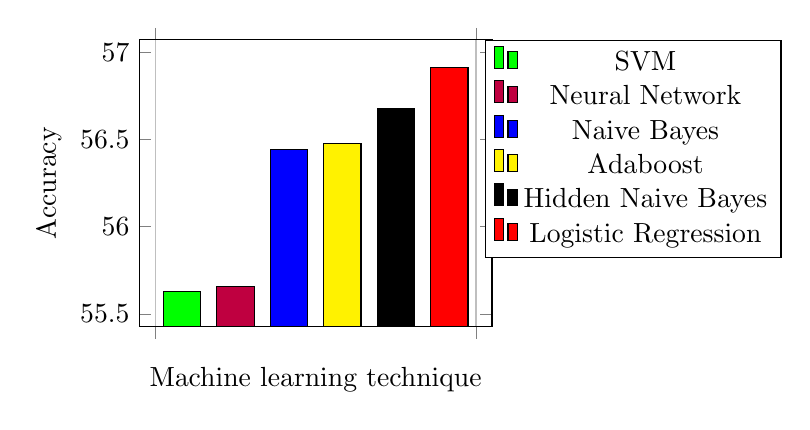
\begin{tikzpicture}
    \begin{axis}[
      %x tick label style={/pgf/number format/1000 sep=},
      xticklabel=\empty,
      ylabel=Accuracy,
      xlabel=Machine learning technique,
      enlargelimits=0.05,
      legend style={at={(1.4,1.0)},
        anchor=north,legend columns=1},
      ybar interval=0.7,
      width=.50\textwidth,
      ymin=55.5, ymax=57,
      reverse legend,
      ]
      \addplot[fill=red] coordinates {(1,56.916) 
        (0,2)
      };
      \addplot[fill=black] coordinates {(1,56.6807) 
        (0,56.6807)
      };
      \addplot[fill=yellow] coordinates {(1,56.479) 
        (0,2)
      };
      \addplot[fill=blue] coordinates {(1,56.4454) 
        (0,56.4454)
      };
      \addplot[fill=purple] coordinates {(1,55.6555) 
        (0,0)
      };
      \addplot[fill=green] coordinates {(1,55.63)
        (0,0)
      };
      \legend{Logistic Regression,Hidden Naive Bayes,Adaboost,Naive Bayes,Neural Network,SVM}
    \end{axis} 
  \end{tikzpicture}
  \caption{Test of best machine learning technique}\label{fig:besttech}
\end{figure}



\subsubsection{Implementation comparison}
To test if Apache Sparks PySpark implementation of logistic regression is implemented properly, it is compared to the equivalent implementations in Weka and R. The data consists of 5000 matches where Weka uses a sparse presentation, while R uses a dense and PySpark the raw file with JSON elements. As seen in \Cref{tab:impl_results}, the implementations are close to equal, the minor differences could be caused by differences in the parameter settings. However these results confirm that all implementations are acceptable and further testing can be performed in any of the environments.

\begin{table}[!htb]
  \centering
  \begin{tabular}{|l|c|}
    \hline
    Implementation  & Accuracy  \\
    \hline
    Weka & 55\%  \\
    R & 55\%\\
    PySpark & 53\%\\ 
    \hline
  \end{tabular}
  \caption{Implementation comparison results}
  \label{tab:impl_results}
\end{table}

\subsubsection{Feature representation test}
Features can be presented in many different ways and this test is constructed to finding the best way to that. The representations that will be tested are the methods presented in \Cref{sec:representationoffeatures}. The test was done on an increasing number of matches with all the different methods to check how they hold up with much data. As the result, shown in \Cref{fig:feat-rep}, indicates, method 1 and 4 are very close, but binary being slightly above ternary majority of the time, which is the reason for us choosing binary.

\begin{figure}[!htb]
  \centering
  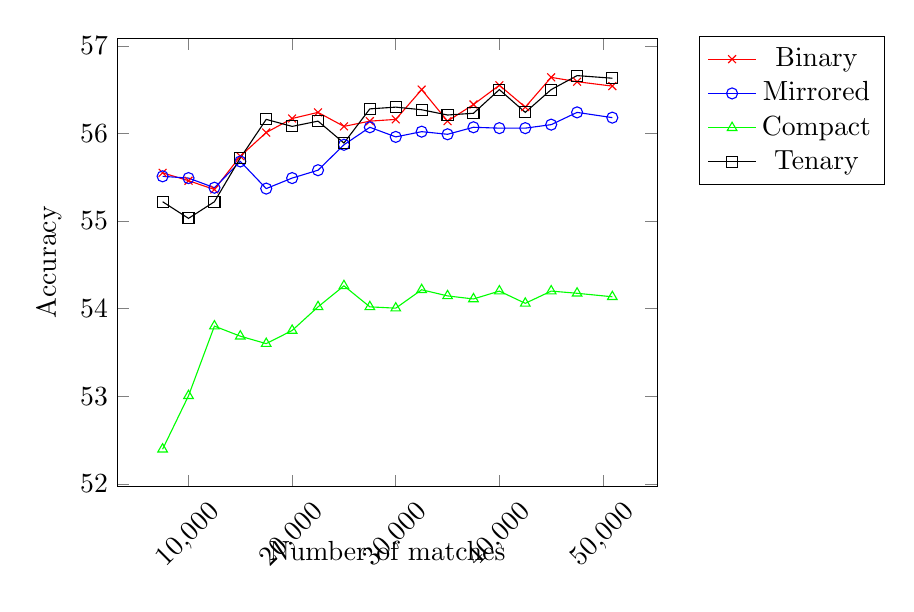
\begin{tikzpicture}[] 
    \begin{axis}[
      xlabel=Number of matches, 
      ylabel=Accuracy,
      xtick={10000,20000,30000,40000,50000},
      xticklabel style={rotate=45,anchor=near xticklabel},
      scaled x ticks=false,
      x label style={at={(axis description cs:0.5,-0.1)},anchor=north},
      legend style={at={(1.25,1.005)},
        anchor=north,legend columns=1},] 
      \addplot[color=red,mark=x] coordinates { 
        (7500, 55.55)
        (10000, 55.46)
        (12500, 55.36)
        (15000, 55.74)
        (17500, 56.01)
        (20000, 56.17)
        (22500, 56.24)
        (25000, 56.08)
        (27500, 56.14)
        (30000, 56.16)
        (32500, 56.50)
        (35000, 56.14)
        (37500, 56.33)
        (40000, 56.55)
        (42500, 56.30)
        (45000, 56.64)
        (47500, 56.59)
        (50901, 56.54)
      };
      \addplot[color=blue,mark=o] coordinates { 
        (7500, 55.51)  
        (10000, 55.49)
        (12500, 55.38)
        (15000, 55.68)
        (17500, 55.37)
        (20000, 55.49)
        (22500, 55.58)
        (25000, 55.87)
        (27500, 56.07)
        (30000, 55.96)
        (32500, 56.02)
        (35000, 55.99)
        (37500, 56.07)
        (40000, 56.06)
        (42500, 56.06)
        (45000, 56.10)
        (47500, 56.24)
        (50901, 56.18)
      };
      \addplot[color=green,mark=triangle] coordinates { 
        (7500, 52.395)  
        (10000, 53.005)
        (12500, 53.80)
        (15000, 53.685)
        (17500, 53.60)
        (20000, 53.75)
        (22500, 54.02)
        (25000, 54.26)
        (27500, 54.02)
        (30000, 54.005)
        (32500, 54.215)
        (35000, 54.145)
        (37500, 54.11)
        (40000, 54.20)
        (42500, 54.06)
        (45000, 54.20)
        (47500, 54.175)
        (50901, 54.135)
      };
      \addplot[color=black,mark=square] coordinates {
        (7500, 55.22)  
        (10000, 55.03)
        (12500, 55.22)
        (15000, 55.72)
        (17500, 56.16)
        (20000, 56.08)
        (22500, 56.14)
        (25000, 55.89)
        (27500, 56.28)
        (30000, 56.30)
        (32500, 56.27)
        (35000, 56.21)
        (37500, 56.23)        
        (40000, 56.50)
        (42500, 56.24)
        (45000, 56.50)
        (47500, 56.66)
        (50901, 56.63)
      };
      \legend{Binary, Mirrored, Compact, Tenary}
    \end{axis} 
  \end{tikzpicture}
  \caption{Test for representation of features}\label{fig:feat-rep}
\end{figure}

\subsubsection{Feature tests}\label{sec:feattest}
Some features might be more expressive than others, and finding the set of features that will yield the best result is imperative. Some more text about \Cref{fig:best-feat}.

\begin{figure}[!htb]
  \centering
  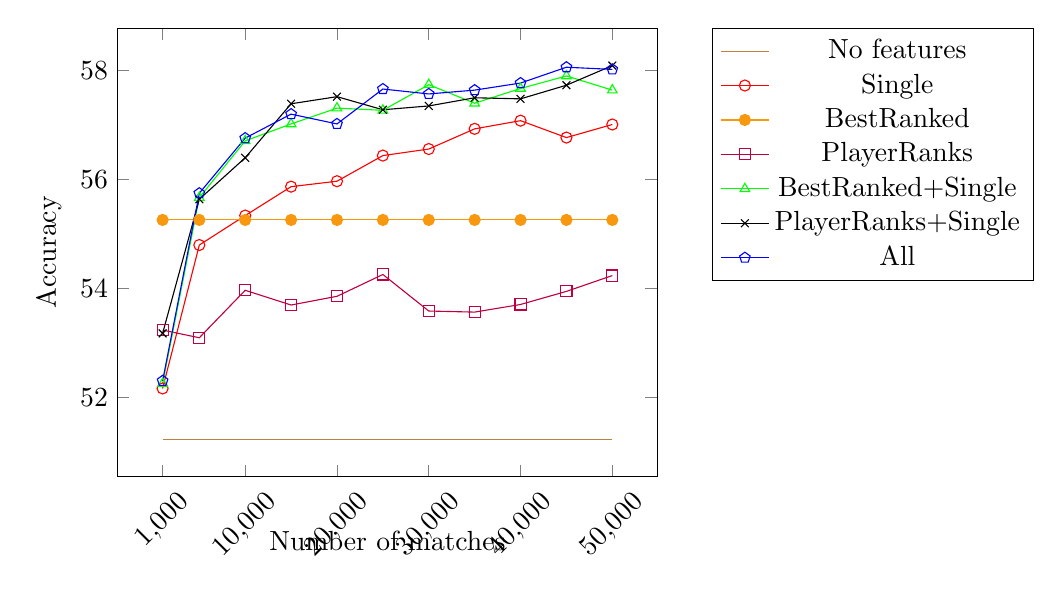
\begin{tikzpicture}[] 
    \begin{axis}[
      xlabel=Number of matches, 
      ylabel=Accuracy,
      xtick={1000,10000,20000,30000,40000,50000},
      xticklabel style={rotate=45,anchor=near xticklabel},
      scaled x ticks=false,
      x label style={at={(axis description cs:0.5,-0.1)},anchor=north},
      legend style={at={(1.4,1.001)},
        anchor=north,legend columns=1},] 
      \addplot[color=brown] coordinates { 
        (1000,51.24)
        (5000,51.24)
        (10000,51.24)
        (15000,51.24)
        (20000,51.24)
        (25000,51.24)
        (30000,51.24)
        (35000,51.24)
        (40000,51.24)
        (45000,51.24)
        (50000,51.24)
      };
      \addplot[color=red,mark=o] coordinates { 
        (1000,52.17)
        (5000,54.8)
        (10000,55.34)
        (15000,55.87)
        (20000,55.97)
        (25000,56.44)
        (30000,56.56)
        (35000,56.93)
        (40000,57.08)
        (45000,56.77)
        (50000,57.01)
      };
      \addplot[color=YellowOrange,mark=*] coordinates { 
        (1000,55.26)
        (5000,55.26)
        (10000,55.26)
        (15000,55.26)
        (20000,55.26)
        (25000,55.26)
        (30000,55.26)
        (35000,55.26)
        (40000,55.26)
        (45000,55.26)
        (50000,55.26)
      };
      \addplot[color=purple,mark=square] coordinates { 
        (1000,53.24)
        (5000,53.1)
        (10000,53.97)
        (15000,53.7)
        (20000,53.86)
        (25000,54.26)
        (30000,53.59)
        (35000,53.57)
        (40000,53.71)
        (45000,53.95)
        (50000,54.24)
      };
      \addplot[color=green,mark=triangle] coordinates { 
        (1000,52.26)
        (5000,55.67)
        (10000,56.71)
        (15000,57.02)
        (20000,57.31)
        (25000,57.27)
        (30000,57.74)
        (35000,57.4)
        (40000,57.67)
        (45000,57.9)
        (50000,57.64)
      };
      \addplot[color=black,mark=x] coordinates { 
        (1000,53.18)
        (5000,55.64)
        (10000,56.4)
        (15000,57.39)
        (20000,57.52)
        (25000,57.28)
        (30000,57.35)
        (35000,57.5)
        (40000,57.48)
        (45000,57.73)
        (50000,58.09)
      };
      \addplot[color=blue,mark=pentagon] coordinates { 
        (1000,52.31)
        (5000,55.75)
        (10000,56.76)
        (15000,57.2)
        (20000,57.02)
        (25000,57.66)
        (30000,57.57)
        (35000,57.64)
        (40000,57.77)
        (45000,58.06)
        (50000,58.02)
      };
      \legend{No features,Single,BestRanked,PlayerRanks,BestRanked+Single,PlayerRanks+Single,All}
    \end{axis} 
  \end{tikzpicture}
  \caption{Accuracy of features}\label{fig:best-feat}
\end{figure}

\subsection{Cluster tests}\label{sec:clustertest}
In this section the tests that requires the cluster. This is due to the size of the tests, and the expected time frame.
\subsubsection{Big data improvements}
To test if big data gives an improvement when predicting the outcome of a match, the same features and method where used on an increasing sized data starting from 1000 matches. After the model was made, it was tested on the training data, as a $\frac{2}{3}$-split and finally cross-validation. And as seen on \Cref{fig:bigdata} there will be more information once more tests has been run!

\begin{figure}[!htb]
  \centering
  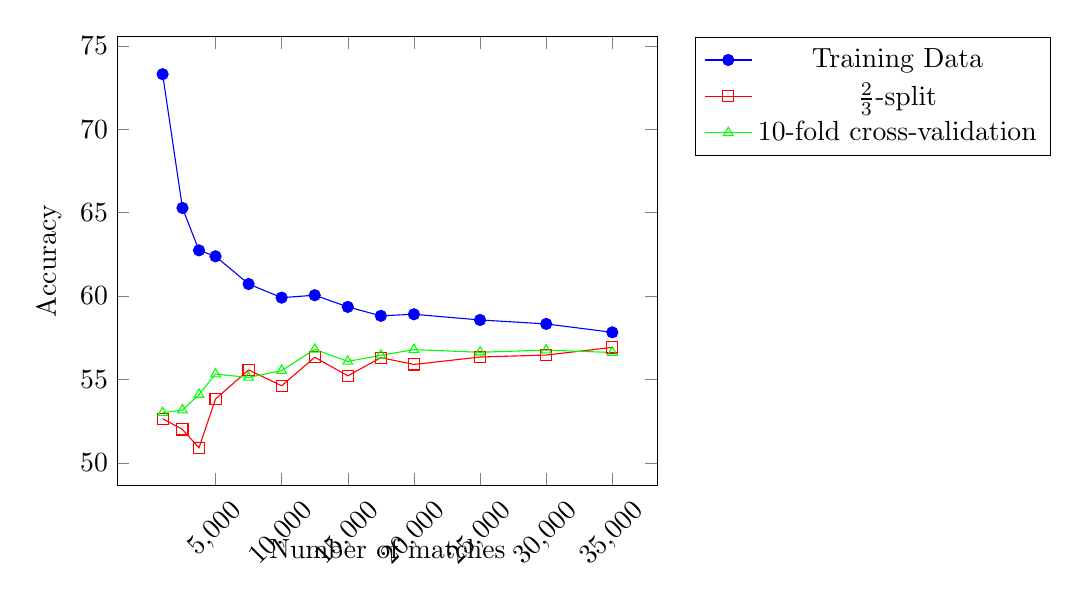
\begin{tikzpicture}[] 
    \begin{axis}[
      xlabel=Number of matches, 
      ylabel=Accuracy,
      xtick={5000,10000,15000,20000,25000,30000,35000},
      xticklabel style={rotate=45,anchor=near xticklabel},
      scaled x ticks=false,
      x label style={at={(axis description cs:0.5,-0.1)},anchor=north},
      legend style={at={(1.4,1.0)},
        anchor=north,legend columns=1},] 
      \addplot[color=blue,mark=*] coordinates {
        (1000, 73.3)   	
        (2500,65.28)  	
        (3750,62.7367)	
        (5000,62.38)
        (7500,60.72)
        (10000,59.9)
        (12500,60.048)
        (15000,59.3467)
        (17500,58.8114)
        (20000,58.905)
        (25000,58.564)
        (30000,58.3267)
        (35000,57.8229)
      };
      \addplot[color=red,mark=square] coordinates {
        (1000,52.6471)
        (2500,52)
        (3750,50.902)
        (5000,53.8235)
        (7500,55.5686)
        (10000,54.6176)
        (12500,56.3294)
        (15000,55.2157)
        (17500,56.3025)
        (20000,55.8971)
        (25000,56.3412)
        (30000,56.4608)
        (35000,56.916)
      };
      \addplot[color=green,mark=triangle] coordinates {
        (1000,53)
        (2500,53.16)
        (3750,54.0944)
        (5000,55.32)
        (7500,55.12)
        (10000,55.53)
        (12500,56.8)
        (15000,56.08)
        (17500,56.4457)
        (20000,56.785)
        (25000,56.628)
        (30000,56.7567)
        (35000,56.6143)
      };
      \legend{Training Data, $\frac{2}{3}$-split, 10-fold cross-validation}
    \end{axis} 
  \end{tikzpicture}
  \caption{Test for representation of features}\label{fig:bigdata}
\end{figure}

\subsubsection{Speed up}
This test is constructed to show that an increasing number of nodes increases the computation speed. As seen in \Cref{sec:clustersetup}, the cluster consists of 4 nodes, this means the test will be run with the master and either 1, 2 or 3 nodes. The data for this test be the same to make the results comparable.

\begin{table}[!htb]
  \centering
  \begin{tabular}{|c|c|}
    \hline
    Number of nodes & Time taken\\
    \hline
    1 & ? \\
    2 & ? \\
    3 & ? \\
    \hline
  \end{tabular}
  \caption{Speed up test results}\label{tab:speedup}
\end{table}

\subsubsection{Prediction with team ranks}
Previous seasons rank for each player is registered in the match data. This test is constructed to test whether this rank alone is a useful feature when predicting a winning team.
\subsubsection{Prediction with all features}
All the features created from the data is used for this test. 
\subsubsection{Prediction with all features except lane}
This test is almost identical to the test seen above, except the lane feature is excluded. This test is performed to learn if the lane each hero choses to defend influences the outcome of the match and if this is actually useful when predicting outcome of future matches.
\subsubsection{Prediction using support vector machine}
The above tests will for this test be performed using support vector machine to see how it compares to logistic regression. 
\subsubsection{Prediction with best features}
The test for prediction with best features will use the features that were determined as the best in \Cref{sec:feattest}. This is done to see how well the prediction can be made at all. This should, should we play the game, give us the opportunity to pick champions that counter those of the opponents team, thus increasing our chances of winning.
\subsubsection{Sample size}
Text.


%%% Local Variables:
%%% mode: latex
%%% TeX-master: "../main"
%%% End:


\section{Conclusion}

\bibliography{Literature}



% APPENDIX
\newpage
\appendix
\section{Setting up Hadoop and Apache Spark}
\label{sec:hadoop}

To get a cluster up and running each machine must first have a \emph{username}, this must have the same name across all machines.
\lstset{language=bash}
\begin{lstlisting}
  adduser ``username''
\end{lstlisting}
For the machines to be able to communicate with the master they need a file with the following content named \emph{hosts}:
\begin{verbatim}
127.0.0.1 localhost

ip node1
ip node2
ip node3
...
\end{verbatim}
Following that each machine needs ssh configured, where \emph{node-id} is the alias created found in the \emph{hosts} file.
\begin{lstlisting}
  ssh-keygen
  ssh-copy-id ``username@node-id''
\end{lstlisting}
This has to be done from master to each slave and from each slave to master.

\subsubsection*{Hadoop}
To set up Hadoop all nodes have to create a hadoop group.
\begin{lstlisting}
  addgroup hadoop
  adduser username hadoop
\end{lstlisting}
At this point Hadoop should be downloaded and installed in the \textsf{/usr/local/hadoop} and then set up the rights.
\begin{lstlisting}
  chown -R username:username /usr/local/hadoop
\end{lstlisting}
The following will be put in \emph{.bashrc} file:
\begin{verbatim}
export JAVA_HOME=/usr/lib/jvm/default-java
export HADOOP_INSTALL=/usr/local/hadoop
export PATH=$PATH:$HADOOP_INSTALL/bin
export PATH=$PATH:$HADOOP_INSTALL/sbin
export HADOOP_MAPRED_HOME=$HADOOP_INSTALL
export HADOOP_COMMON_HOME=$HADOOP_INSTALL
export HADOOP_HDFS_HOME=$HADOOP_INSTALL
export YARN_HOME=$HADOOP_INSTALL
\end{verbatim}
In the file \emph{hadoop-env.sh} found in \textsf{/usr/local/hadoop/etc/hadoop/} the line \emph{JAVA\_HOME} should be replaced with \emph{export JAVA\_HOME=/usr/lib/jvm/default-java}.
In addition the \emph{core-site.xml} which is found in \textsf{/usr/local/hadoop/etc/hadoop/} needs an added property: 
\begin{verbatim}
<property>
  <name>fs.defaultFS</name>
  <value>hdfs://MASTER:9000</value>
</property>
\end{verbatim}
\emph{MASTER} needs to be replaced with the hostname for the master node.

Another file that needs added properties is \emph{hdfs-site.xml}, which can be found in the folder \textsf{/usr/local/hadoop/etc/hadoop/}:
\begin{verbatim}
<property>
  <name>dfs.namenode.data.dir</name>
  <value>file:/home/username/data/hdfs/namenode</value>
</property>

<property>
  <name>dfs.datanode.data.dir</name>
  <value>file:/home/username/data/hdfs/datanode</value>
</property>
\end{verbatim}
The final thing that needs for Hadoop to run is for the master to know the slaves. Create a file \emph{slaves} in \textsf{/usr/local/hadoop/etc/hadoop/} with all the hostnames of slaves listed:
\begin{verbatim}
node1
node2
...
\end{verbatim}

\subsubsection*{Apache Spark}
To get spark running download and install it to \textsf{/usr/local/spark} and again run the command to set up the correct rights.
\begin{lstlisting}
  chown -R username:username/usr/local/spark
\end{lstlisting}
The final step for setting up Apache Spark is copying the \emph{slaves} file into the folder \textsf{/usr/local/spark/conf/}.


\subsubsection*{Starting the cluster}
To start the cluster the master has to run the following commands:
\begin{lstlisting}
  start-dfs.sh
  cd /usr/local/spark
  ./sbin/start-all.sh
\end{lstlisting}
Now the cluster is ready to use.

\subsubsection*{Using the cluster}
WE MIGHT NEED STUFF HERE!

%%% Local Variables:
%%% mode: latex
%%% TeX-master: "../main"
%%% End:

\begin{frame}{title}
\begin{itemize}
\item item1
\begin{itemize}
\item item2
\end{itemize}
\end{itemize}
\vspace{20cm}
\end{frame}
\section{Data and Feature Setup}\label{sec:features}
In \Cref{sec:matchdata} we investigate the match data made available by the RGs API, which covers almost any detail of a given LoL match.
\Cref{sec:choosingfeatures} identifies a number of features that can be extracted from match data, which we think are most important when it comes to prediction of the winning team. The choice is based on our intuition as more or less experienced LoL players. The size of each type of features domain is calculated in \Cref{sec:featuresparsity}, as well as the sparsity with regards to how many features that appear in each match.
In \Cref{sec:representationoffeatures}, a possible feature symmetry issue is investigated which raises a number of concerns and suggestions for solutions as to how the extracted features should be represented. 


\subsection{League of Legends Match Information}\label{sec:matchdata}
Riot Games records large amounts of information about played matches as well as the players~\cite{matchinfo}. Much, if not all, of this data is publicly available through their online API. In this paper the focus will be on the match data only, and more particularly the data that can be extracted before a match starts. The only exception is information about which team that won each match. Since we want to predict who wins, we need that data to train and evaluate a classifier.
We have chosen to extract the following data from each match:
\begin{itemize}
\item The team that won the match.
\item The champions on each of the two teams.
\item The rank of all players in the match.
\item The lane played by each player.
\item The runes used by each player.
\item The masteries used by each player.
\item The summoner spells used by each player.
\item The game mode of the match.
\item The queue type of the match.
\end{itemize}

All the extracted information has be chosen because we think it might be useful for estimating how good a particular team is against another team.
The champions on each of the two teams have been included because some champions may be better than other.
The rank of players are considered because the rank system in LoL aims to assign better players a greater rank.
Intuitively, a team of high ranked players must be better than a team of low ranked players.
The lane played by each player may be useful, because players often stick to one particular \textit{lane} for the first half a match.
Note that the lanes of the opponent team is not known before the game starts, but we have still chosen to include it, because it very often can determined based on the picked champions. Knowing the lane of the players means knowing the ranks and champion of the players that most often fights against each other.
The masteries and runes are worth knowing, because each of them improve some property of a champion. 
The summoner spells are also worth considering because they adds additional properties to a champion.
Different game modes imply different play styles. By only considering the 5v5 game mode (where two teams of 5 players fight each other), we hope to achieve better predictions.
The queue type of the match lets us know if the LoL match making system has formed the two teams, or the players have formed the two teams themselves.
Teams formed on their own may be better, because the players in self formed teams often know each other better and more often use voice communication tools.
Finally the matches patch version is used to make sure that we only use matches from the same patches. Different patches change many aspects of the game, e.g. the strength of particular champions, and without accounting for different patches, the trained classifier accuracy may decrease.  

The data set we use use consists of matches played from $23^{\text{rd}}$ of March 2015 to $27^{\text{th}}$ of March 2015. It includes match details for matches played across the world. When filtering the games to include only 5v5 game modes, we are left with 1925980 matches. The patch version of all matches used is $5.6$.



\end{document}

%%% Local Variables:
%%% mode: latex
%%% TeX-master: t
%%% End:
